\subsubsection{Navigation}
\paragraph{TabNavigator} Der \GLS{TabNavigator} ist die Navigationsleiste unten am Bildschirm. Damit kann die anwendende Person zwischen verschiedenen Ansichten wechseln. Die Ansicht, auf der man sich gerade befindet, wird mit einem Farbton hervorgehoben. Die Abbildung \ref{fig:bottomtab} zeigt die \GLS{BottomTabBar} der entwickelten App. \citev{tabnavigator}

\begin{figure}[H]
    \centering
    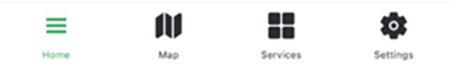
\includegraphics[width=0.4\textwidth]{images/tab.png}
    \caption{BottomTab der App}
    \label{fig:bottomtab}
\end{figure}

\paragraph{StackNavigator}Beim \Gls{StackNavigator} wird eine Seite auf die aktuelle Seite gelegt. Dadurch ist es möglich, mehrere Seiten aufeinander zu stapeln. Mit dem Klicken auf die Rücktaste (im Beispiel auf der Abbildung \ref{fig:appheader} ist es der Schriftzug „Map“) gelangt man auf den vorherigen Screen zurück. \citev{stacknavigator}

\begin{figure}[H]
    \centering
    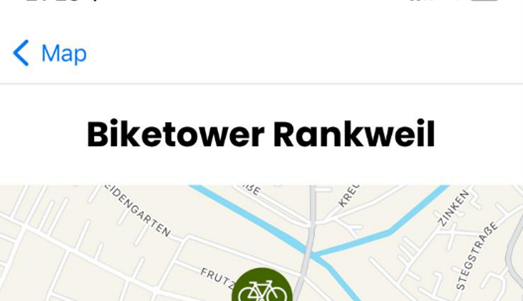
\includegraphics[width=0.35\textwidth]{images/appheader.png}
    \caption{Header der App mit Rücktaste}
    \label{fig:appheader}
\end{figure}


Die Navigation der App besteht aus einem Bottom\GLS{TabNavigator}. Dieser führt zu vier verschiedenen \Gls{StackNavigator}:

\begin{itemize}
    \item HomeStack
    \item MapStack
    \item ServiceStack
    \item SettingsStack
\end{itemize}

\begin{figure}[H]
    \centering
    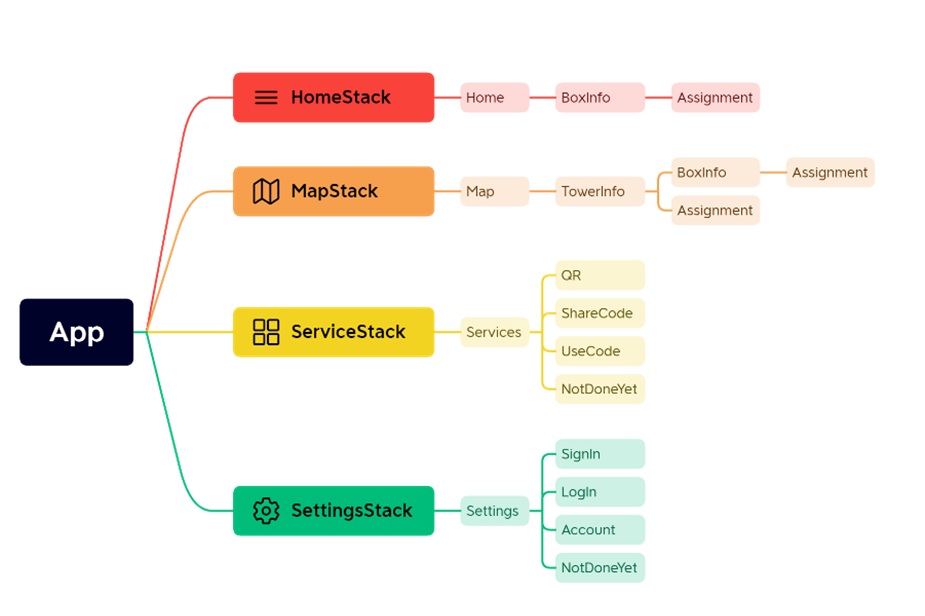
\includegraphics[width=1\textwidth]{images/appnavigation.png}
    \caption{Navigations-Struktur der App}
    \label{fig:appnavigation}
\end{figure}

Die Abbildung \ref{fig:appnavigation} zeigt die Navigations-Struktur der App. Grundsätzlich kann man über die \GLS{BottomTabBar} von einem \GLS{StackNavigator} zu einem anderen navigieren. Bei jedem Stack wird der erste Screen angezeigt. Von dort aus kann man auf eine oder mehrere Unterseiten gelangen.